\begin{frame}<handout: 0>[t,fragile]{Eine einfache Funktion} % Version 1
\begin{lstlisting}
public double f ( double x ) {
   if( x < 5.0 ) return 3.0;
   else if( x < 10.0 ) return 2.0;
   else return 4.0;
}
\end{lstlisting}
~ \\[-.5em]
\begin{minipage}[t]{3.5cm}
\only<2->{
Beispielwerte für f:

~ \\
\begin{tabular}{|c|c|}
\textbf{x} & \textbf{f( x )}  \\ \hline
1 & 3  \\
3 & 3  \\
7 & 2  \\
12 & 4
\end{tabular} 
}
\end{minipage} 
\hfill

\end{frame}

\begin{frame}[t,fragile]{Eine einfache Funktion} % Version 2
\begin{lstlisting}
public double f ( double x ) {
   if( x < 5.0 ) return 3.0;
   else if( x < 10.0 ) return 2.0;
   else return 4.0;
}
\end{lstlisting}
~ \\[-.5em]
\begin{minipage}[t]{3.5cm}
Beispielwerte für f:

~ \\
\begin{tabular}{|c|c|}
\textbf{x} & \textbf{f( x )}  \\ \hline
1 & 3  \\
3 & 3  \\
7 & 2  \\
12 & 4
\end{tabular} 
\end{minipage} 
\hfill
\begin{minipage}[t]{7cm}
Unit-Tests für f:

\begin{lstlisting}
@Test public void valuesOfF() {
  assertEquals( 3.0, f( 1.0 ), 0.01 );
  assertEquals( 3.0, f( 3.0 ), 0.01 );
  assertEquals( 2.0, f( 7.0 ), 0.01 );
  assertEquals( 4.0, f( 12.0 ), 0.01 );
}
\end{lstlisting}
\end{minipage}

\end{frame}

\begin{frame}[t,fragile]{Eine einfache Funktion} % Version 3
\begin{lstlisting}
public double f ( double x ) {
   if( x < 5.0 ) return 3.0;
   else if( x < 10.0 ) return 2.0;
   else return 4.0;
}
\end{lstlisting}
~ \\[-.5em]
\begin{minipage}[t]{3.5cm}
Beispielwerte für f:

~ \\
\begin{tabular}{|c|c|}
\textbf{x} & \textbf{f( x )}  \\ \hline
1 & 3  \\
3 & 3  \\
7 & 2  \\
12 & 4
\end{tabular} 
\end{minipage} 
\hfill
\begin{minipage}[t]{5.5cm}
~ \\
\vspace{-2em}\\
\only<1| handout:0>{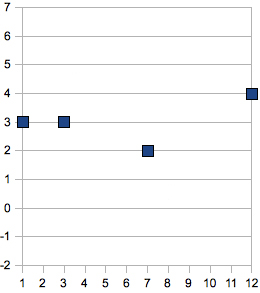
\includegraphics[height=4.5cm]{0Funktionen.jpg}}
\only<2| handout:0>{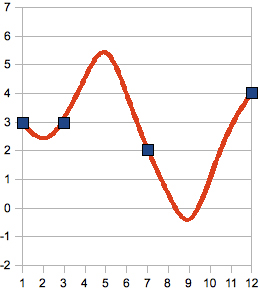
\includegraphics[height=4.5cm]{1Funktion.jpg}}
\only<3| handout:0>{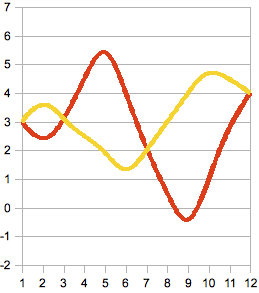
\includegraphics[height=4.5cm]{2Funktionen.jpg}}
\only<4>{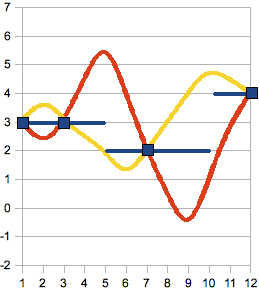
\includegraphics[height=4.5cm]{3Funktionen.jpg}}
\end{minipage}

\end{frame}

\begin{frame}{Was ist das Problem?}

\glqq{}Traditional test suites verify a few well-picked scenarios or example inputs. However, such example-based testing does not uncover errors in legal inputs that the test writer overlooked.\grqq{}

\hfill[Saff et.al.]

\end{frame}

\begin{frame}{Eine Alternative: Spezifikationen}
Eine geeignete mathematische Spezifikation ist z.\,B.:
\begin{eqnarray*}
\forall x. \; \parbox{2cm}{$(x < 5$} &\Rightarrow& f(x) = 3) \\
\land \; \parbox{2cm}{$(5 \leq x < 10$} &\Rightarrow& f(x) = 2)\\
\land \; \parbox{2cm}{$(10 \leq x$} &\Rightarrow& f(x) = 4)
\end{eqnarray*}
\end{frame}

% \begin{frame}

% \glqq{}A theory generalizes a (possibly infinite) set of example-based
% tests. A theory is an assertion that should be true for any data, and
% it can be exercised by human-chosen data or by automatic data
% generation.\grqq

% \hfill[Saff et.al.]

% \end{frame}

\begin{frame}{Eine Lösung: JUnit Theories}
	\begin{itemize}
		\item Herkömmliche Tests benutzen Beispiele:
			\begin{itemize}
				\item Überprüfung des Verhaltens unter ausgewählten Eingaben
				\item Entwickler ist dafür verantwortlich, charakteristische Beispiele zu wählen
			\end{itemize}
		\item Eine Theory verallgemeinert eine Menge von Tests:
			\begin{itemize}
				\item Vorbedingung wird explizit angegeben
				\item Assertion muss für alle Eingaben gelten, die die Vorbedingungen erfüllen
			\end{itemize}
	\end{itemize}
\end{frame}


% \begin{frame}{Theories -- Wie sehen sie genau aus?}
% 	\begin{itemize}
% 		\item Neu seit JUnit Version 4.4
% 		\item Parametrisierte Testmethode mit Vorbedingungen (Assumptions)
% 			\begin{itemize}
% 				\item \texttt{assumeThat()}
% 				\item \texttt{assumeTrue()}
% 				\item \texttt{assumeNotNull()}
% 			\end{itemize}
% 		\item \texttt{@Theory} statt \texttt{@Test}
% 		\item Input für Testmethoden über \texttt{@DataPoint}(\texttt{s})-Annotation
% 	\end{itemize}
% \end{frame}


\begin{frame}[fragile]{Theories für unsere Funktion}
\begin{lstlisting}
@Theory
public void valuesLessThan5( double x ) {
   assumeTrue( x < 5.0 );
   assertEquals( 3.0, f(x), 0.01 );
}

@Theory
public void valuesBetween5And10( double x ) {
   assumeTrue( 5.0 <= x ); 
   assumeTrue( x < 10.0 );
   assertEquals( 2.0, f(x), 0.01 );
}

@Theory
public void values10OrGreater( double x ) {
   assumeTrue( 10.0 <= x );
   assertEquals( 4.0, f(x), 0.01 );
}
\end{lstlisting}
\end{frame}

\begin{frame}[fragile]{Woher kommen die Eingabewerte?}
\begin{lstlisting}
@DataPoint
public static double VALUE1 = 1.0;

@DataPoint
public static double VALUE2 = 3.0;

@DataPoint
public static double VALUE3 = 7.0;

@DataPoint
public static double VALUE4 = 12.0;
\end{lstlisting}
\end{frame}

\begin{frame}{}
\begin{center}
DEMO
\end{center}
\end{frame}

\begin{frame}[fragile]{ScalaCheck}
	\begin{itemize}
		\item Generatoren erzeugen randomisierte Testwerte
		\item Test ist grün nach 100 erfolgreichen Durchläufen
		\item Test ist rot nach 500 unpassenden Eingaben
	\end{itemize}
\end{frame}

\begin{frame}
\begin{center}\Huge
Das war's!
\end{center}
\pause
\vspace{.1cm}
\begin{flushright}\Huge
\itshape Wirklich?
\end{flushright}
\end{frame}
